\documentclass{beamer}
\usepackage{listings}
\lstset{
%language=C,
frame=single, 
breaklines=true,
columns=fullflexible
}
\usepackage{subcaption}
\usepackage{url}
\usepackage{commath}
\usepackage{tikz}
\usepackage{pgfplots}
\pgfplotsset{compat=1.17}
\usepackage{tkz-fct}
\usepackage{mathrsfs}
\usepackage{txfonts}
\usepackage{tkz-euclide} 
\usetikzlibrary{calc,math}
\usepackage{float}
\providecommand{\brak}[1]{\ensuremath{\left(#1\right)}}
\renewcommand{\vec}[1]{\mathbf{#1}}
\providecommand{\pr}[1]{\ensuremath{\Pr\left(#1\right)}}
\usepackage[export]{adjustbox}
\usepackage[utf8]{inputenc}
\usepackage{amsmath}
\usetheme{Boadilla}
\title{Research Paper Presentation}
\author{Ayush Jha - CS20BTECH11006}

\begin{document}
\begin{frame}
\titlepage
\end{frame}

\begin{frame}{Gaussian Mixture Model for Estimating Solar Irradiance Probability Density}
\begin{block}{Abstract}
\begin{enumerate}
    \item The increasing need for photovoltaic generation resources 
    demands power network designers to obtain accurate estimates of solar irradiance at a given site. 
    \item The current parametric Beta distribution can be problematic and may lead to model mis-specification. 
    \item The paper proposes Gaussian Mixture Model (GMM) as a more robust estimation of solar irradiance probability density at a certain site.
    \item Multi-year solar data from eight locations in the United States is utilized to evaluate the accuracy of the GMM estimate and compare its performance with the popular Beta distribution.
\end{enumerate}
\end{block}
\end{frame}
\begin{frame}{Definitions}
    \begin{block}{Probability Density Estimation}
    Using the observations in a random sample to estimate the general density of probabilities beyond just the sample of data is known as Probability Density Estimation.
    \end{block}
    \begin{block}{Solar Irradiance }
    The solar irradiance is the output of light energy from the entire disk of the Sun, measured at the Earth. 
    \end{block}
    \begin{block}{Gaussian distribution}
    Gaussian distribution (also known as normal distribution) is a continuous probability distribution for a real-valued random variable with a  bell-shaped curve.
    \end{block}
\end{frame}
\begin{frame}{Definitions}
\begin{block}{Gaussian PDF}
 \begin{align}
        f_X(x) = \dfrac{1}{\sigma \sqrt{2\pi}}\exp{-\dfrac{1}{2} \brak{\dfrac{x-\mu}{\sigma}}^2}
    \end{align}
    with $ \sigma $ as standard deviation and $ \mu$ as mean.
\end{block}  
\begin{block}{Gaussian Mixture Model}
 A Gaussian mixture model is a probabilistic model that assumes all the data points are generated from a mixture of a finite number of Gaussian distributions with unknown parameters.
\end{block}
\end{frame}
\begin{frame}{The Beta Probability Density Function}
\begin{block}{Introduction}
\begin{enumerate}
    \item The Beta distribution is the most common parametric family of probability distributions used to estimate the probability density of Normalized Solar Irradiance (NSI) data.
    \item However, the use of a simple parametric distribution (such as the Beta distribution) can possibly lead to the risk of mis-specification of the model and can result in wrong planning decisions.
    \item It is also used for research works on network planning and design, distribution system partitioning into microgrids, and voltage stability for networks with distributed generation, etc.
\end{enumerate}
\end{block}
\end{frame}

\begin{frame}{The Beta Probability Density Function}
    \begin{block}{PDF}
\begin{align}
    f_{Beta}(x) &= \dfrac{\Gamma(\alpha + \beta)}{\Gamma(\alpha)\Gamma(\beta)}x^{\alpha-1}(1-x)^{\beta-1}
\end{align}
where $ x\in (0,1)$, $ \Gamma $ is the gamma function, and $ \alpha, \beta \in (0, \infty)$ are the first and second shape parameters respectively, given by,
\begin{align}
    \alpha & = \dfrac{\gamma \times \beta}{1- \gamma} \\
    \beta & = (1- \gamma) \brak{\dfrac{\gamma(1-\gamma)}{\sigma^2}-1}
\end{align}
where $ \sigma$ and $\gamma $ are the standard deviation and mean of the random variable, respectively.
\end{block}
\end{frame}

\begin{frame}{Gaussian Mixture Model}
\begin{block}{Introduction}
\begin{enumerate}
    \item  To overcome the limitations by Beta distribution, recent works have suggested
new models for estimating solar irradiance based on a non-parametric approach.
   \item In this paper, the GMM is proposed for estimating solar irradiance probability density as
a more accurate alternative to the Beta distribution.
\item The GMM is a finite convex linear combination of Gaussian densities with different parameters of each probability density. 
\item  The careful selection of a correct number of mixture components is of top importance when fitting a finite mixture distribution. 
\end{enumerate}
\end{block}
\end{frame}
\begin{frame}{Gaussian Mixture Model}
    \begin{block}{Details of model}
    \begin{enumerate}
        \item The Expectation–Maximization (EM) framework ( advanced iterative clustering technique) 
        is adopted in this paper to obtain an estimation of the parameters of the GMM PDF.
        \item The Bayesian Information Criterion (BIC) approach is considered to determine the number
of components in an optimal manner.
\item The probability density distribution of the GMM can approximate any arbitrarily shaped non-Gaussian density
    \end{enumerate}
    \end{block}
\end{frame} 
\begin{frame}{Gaussian Mixture Model}
    \begin{block}{PDF}
    Suppose that the observed solar irradiance values are denoted by $x = x_1, \cdots ,x_n $ , and let the $j^{th}$ entry of the random variable be modeled as a linear combination of Gaussian densities then,
\begin{align}
f_X(x_j | \theta) = \sum_{i=1}^{C}w_i \phi(x_i, \theta_i) \text{ , } x_j \ge 0 \text{ , } j=1, \cdots N
\end{align}
where $C$ is the number of mixture components, and each $i^{th}$ component is given by
\begin{align}
    \phi(x_i, \theta_i) = \dfrac{1}{\sqrt{2\pi\sigma_i^2}}\exp{\brak{- \dfrac{(x_j- \mu_i)^2}{2\sigma_i^2}}}
\end{align}
where its weight is $w_i > 0$, with $\sum_{i=1}^{C}w_i =1$. The parameters $ \sigma_i^2$ and $ \mu _i$ correspond to the variance and mean of the $ i^{th}$ mixture component.
    \end{block}
\end{frame}
\begin{frame}{Results and Performance evaluations }

\begin{block}{Introduction}
\begin{enumerate}
    \item The robustness of the proposed GMM and common Beta distributions for characterizing the variability of solar data of eight cities is assessed in this section.
    \item The solar data had the mean and varince of the solar irradiance values for all eight cities.
    \item  The proposed GMM routine was coded in MATLAB with the PDF parameters computed using the EM algorithm and the optimal number of mixture components found using the BIC approach.
    \item  The Beta distribution shape parameters and density estimates were computed in MATLAB using the functions betafit and betapdf. 
\end{enumerate}
\end{block}
\end{frame}

\begin{frame}{Results and Performance evaluations }
    \begin{figure}
    \centering
    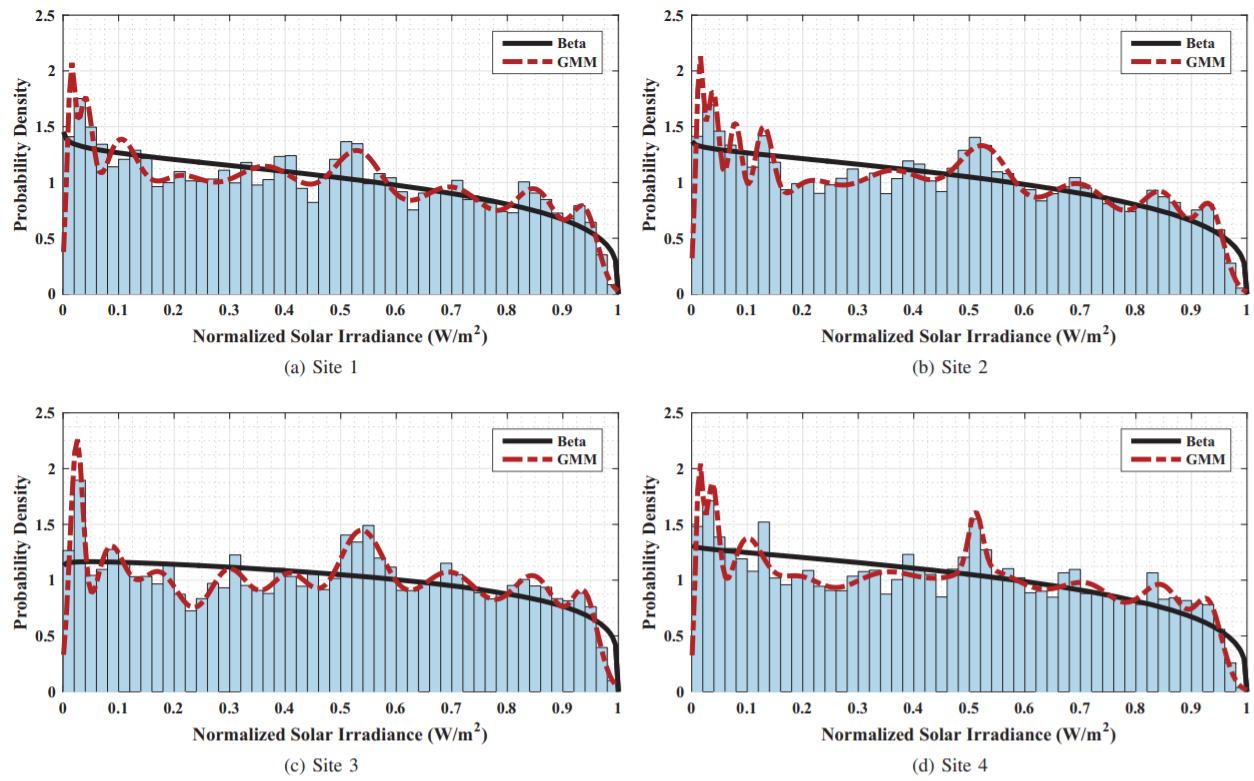
\includegraphics[width=0.9\columnwidth]{1.png}
    \caption{Probability Density plots and Histograms (sites 1-4)}
    \label{fig:1}
\end{figure}
\end{frame}
\begin{frame}{Results and Performance evaluations }
     \begin{figure}
    \centering
    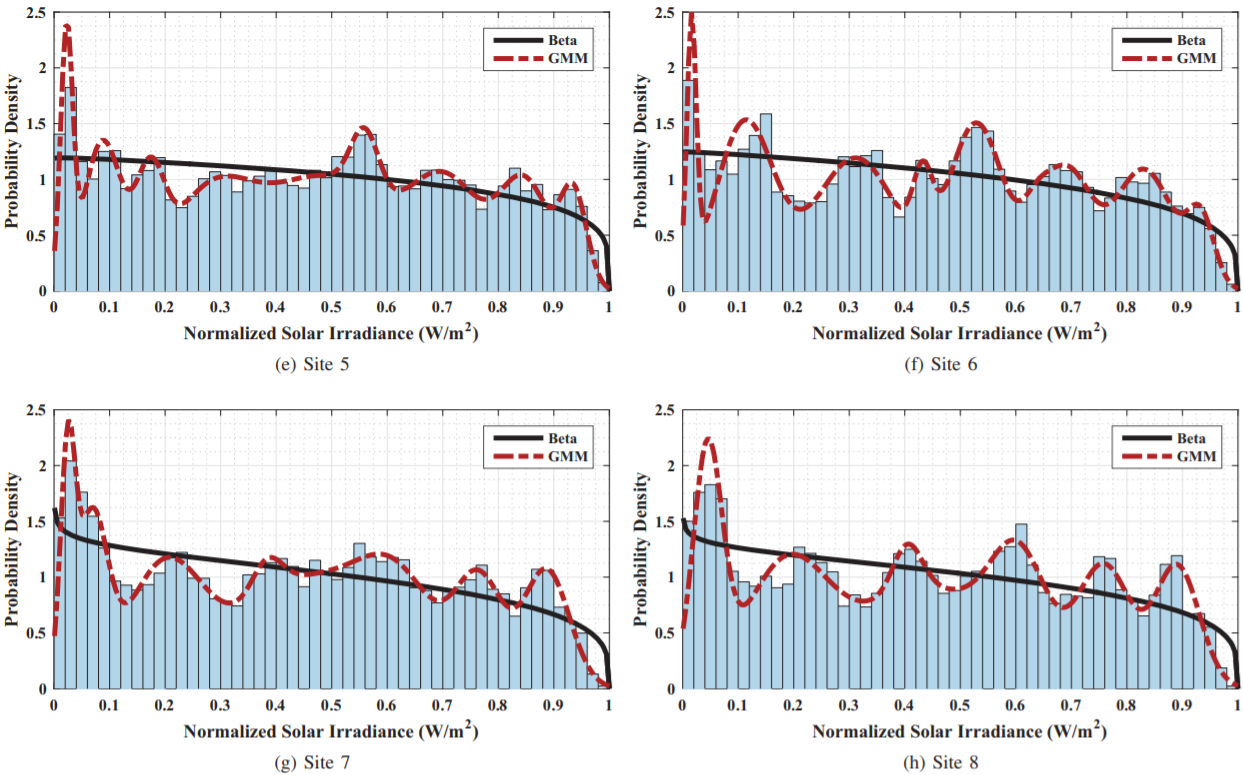
\includegraphics[width=0.9\columnwidth]{2.png}
    \caption{Probability Density plots and Histograms (sites 5-8)}
    \label{fig:2}
\end{figure}
\end{frame}
\begin{frame}{Results and Performance evaluations }
\begin{block}{Analysing Figures}
    \begin{enumerate}
        \item Figures \ref{fig:1} and \ref{fig:2} shows the normalized histograms (with density scaling) of NSI data at the eight selected sites, overlaid with the two density estimates.
        \item Visually, these plots show substantial discrepancies between the data histogram and the Beta distribution.
\item  As depicted, the proposed GMM provides a more accurate estimate of NSI probability density.
    \end{enumerate}
\end{block}
     \begin{block}{Theoretical Performance measures}
    \begin{enumerate}
        \item Coefficient of determination, $R^2$ index
        \item A goodness-of-fit test: the Kolmogorov–Smirnov (K–S) test
\item Three standard error measures: Mean Absolute Error (MAE), Mean Absolute Percentage Error (MAPE), and Root Mean Square Error (RMSE). 
    \end{enumerate}
    \end{block}
\end{frame}
\begin{frame}{Results and Performance evaluations }
    \begin{block}{K-S test}
    \begin{enumerate}
        \item  Each K–S test returns a p-value which, informally, is a measure of the evidence against the null hypothesis.
        \item When the observed data set does not provide sufficient evidence validating the hypothesis that it is associated with the statistical model, the K–S test rejects the null hypothesisat the $ \alpha_{K-S}$ significance level.
        \item The proposed BIC-assisted GMM applying the EM algorithm produces p-values which indicate a failure to reject the null hypothesis at the $ \alpha_{K-S}$ significance level for all sites.
\item This suggests that the proposed model is a more robust approach for estimating solar GHI data.
    \end{enumerate}
    \end{block}
\end{frame}
\begin{frame}{Results and Performance evaluations }
    \begin{block}{Formulas}
    In addition to the goodness-of-fit test, the performance of the proposed GMM PDF is evaluated against $f_{Beta}$ using the $R^2$ index, and three standard measures: MAE, MAPE and RMSE given by
\begin{align}
    R^2 &= 1- \dfrac{\sum_{i=1}^{t}(y_i-\hat{y_i})^2}{\sum_{i=1}^{t}(y_i-\Bar{y})^2} \\
    MAE &= \dfrac{1}{t} \sum_{i=1}^{t}\abs{y_i-\hat{y_i}}\\
    MAPE &= \dfrac{1}{t} \sum_{i=1}^{t} \abs{\dfrac{y_i-\hat{y_i}}{y_i}}\\
    RMSE &= \sqrt{ \dfrac{1}{t} \sum_{i=1}^{t} (y_i-\hat{y_i})^2}
\end{align}    
    \end{block}
\end{frame}
\begin{frame}{Results and Performance evaluations }
\begin{block}{Formulas contd.}
where t is the number of data bins chosen using the square root rule, $ y_i$ is the probability of solar GHI data being within bin i calculated from the data set, $\hat{y_i}$ is the probability within the
same bin calculated from the estimated data set, $ \Bar{y} =  \dfrac{1}{t}\sum_{i=1}^{t} y_i$ and $ i=1,2,\cdots ,t$.
\end{block}
    \begin{block}{Result}
    \begin{enumerate}
        \item The computed values of  $R^2$, MAE, MAPE and RMSE values with error percentage improvements computed with respect to the Beta distribution for all sites.
        \item The proposed GMM produces the highest $ R^2$ indices and the lowest error values for all eight sites.
        \item So this shows that the GMM is a more robust estimate than the popular Beta distribution for
        estimating solar irradiance probability density.
    \end{enumerate}
    
    \end{block}
\end{frame}
\begin{frame}{Conclusion}
    \begin{block}{Points}
    \begin{enumerate}
        \item A Gaussian Mixture Model (GMM) is proposed in this paper for estimating solar irradiance probability density at a given site. 
\item The proposed GMM parameters are obtained using the Expectation–Maximization (EM) algorithm 
\item The optimal number of mixture components is determined using the Bayesian Information Criterion (BIC).
\item The proposed GMM produces the best performance metrics and the highest percentage improvements providing a more accurate estimation of solar irradiance compared with the popular Beta distribution.
    \end{enumerate}
    \end{block}
\end{frame}
\end{document}